\documentclass[
  jou,
  floatsintext,
  longtable,
  a4paper,
  nolmodern,
  notxfonts,
  notimes,
  colorlinks=true,linkcolor=blue,citecolor=blue,urlcolor=blue]{apa7}

\usepackage{amsmath}
\usepackage{amssymb}



\usepackage[bidi=default]{babel}
\babelprovide[main,import]{spanish}
\StartBabelCommands{spanish}{captions} [unicode, fontenc=TU EU1 EU2, charset=utf8] \SetString{\keywordname}{Palabras
Claves}
\EndBabelCommands


% get rid of language-specific shorthands (see #6817):
\let\LanguageShortHands\languageshorthands
\def\languageshorthands#1{}

\RequirePackage{longtable}
\RequirePackage{threeparttablex}

\makeatletter
\renewcommand{\paragraph}{\@startsection{paragraph}{4}{\parindent}%
	{0\baselineskip \@plus 0.2ex \@minus 0.2ex}%
	{-.5em}%
	{\normalfont\normalsize\bfseries\typesectitle}}

\renewcommand{\subparagraph}[1]{\@startsection{subparagraph}{5}{0.5em}%
	{0\baselineskip \@plus 0.2ex \@minus 0.2ex}%
	{-\z@\relax}%
	{\normalfont\normalsize\bfseries\itshape\hspace{\parindent}{#1}\textit{\addperi}}{\relax}}
\makeatother




\usepackage{longtable, booktabs, multirow, multicol, colortbl, hhline, caption, array, float, xpatch}
\usepackage{subcaption}
\renewcommand\thesubfigure{\Alph{subfigure}}
\setcounter{topnumber}{2}
\setcounter{bottomnumber}{2}
\setcounter{totalnumber}{4}
\renewcommand{\topfraction}{0.85}
\renewcommand{\bottomfraction}{0.85}
\renewcommand{\textfraction}{0.15}
\renewcommand{\floatpagefraction}{0.7}

\usepackage{tcolorbox}
\tcbuselibrary{listings,theorems, breakable, skins}
\usepackage{fontawesome5}

\definecolor{quarto-callout-color}{HTML}{909090}
\definecolor{quarto-callout-note-color}{HTML}{0758E5}
\definecolor{quarto-callout-important-color}{HTML}{CC1914}
\definecolor{quarto-callout-warning-color}{HTML}{EB9113}
\definecolor{quarto-callout-tip-color}{HTML}{00A047}
\definecolor{quarto-callout-caution-color}{HTML}{FC5300}
\definecolor{quarto-callout-color-frame}{HTML}{ACACAC}
\definecolor{quarto-callout-note-color-frame}{HTML}{4582EC}
\definecolor{quarto-callout-important-color-frame}{HTML}{D9534F}
\definecolor{quarto-callout-warning-color-frame}{HTML}{F0AD4E}
\definecolor{quarto-callout-tip-color-frame}{HTML}{02B875}
\definecolor{quarto-callout-caution-color-frame}{HTML}{FD7E14}

%\newlength\Oldarrayrulewidth
%\newlength\Oldtabcolsep


\usepackage{hyperref}



\usepackage{color}
\usepackage{fancyvrb}
\newcommand{\VerbBar}{|}
\newcommand{\VERB}{\Verb[commandchars=\\\{\}]}
\DefineVerbatimEnvironment{Highlighting}{Verbatim}{commandchars=\\\{\}}
% Add ',fontsize=\small' for more characters per line
\usepackage{framed}
\definecolor{shadecolor}{RGB}{241,243,245}
\newenvironment{Shaded}{\begin{snugshade}}{\end{snugshade}}
\newcommand{\AlertTok}[1]{\textcolor[rgb]{0.68,0.00,0.00}{#1}}
\newcommand{\AnnotationTok}[1]{\textcolor[rgb]{0.37,0.37,0.37}{#1}}
\newcommand{\AttributeTok}[1]{\textcolor[rgb]{0.40,0.45,0.13}{#1}}
\newcommand{\BaseNTok}[1]{\textcolor[rgb]{0.68,0.00,0.00}{#1}}
\newcommand{\BuiltInTok}[1]{\textcolor[rgb]{0.00,0.23,0.31}{#1}}
\newcommand{\CharTok}[1]{\textcolor[rgb]{0.13,0.47,0.30}{#1}}
\newcommand{\CommentTok}[1]{\textcolor[rgb]{0.37,0.37,0.37}{#1}}
\newcommand{\CommentVarTok}[1]{\textcolor[rgb]{0.37,0.37,0.37}{\textit{#1}}}
\newcommand{\ConstantTok}[1]{\textcolor[rgb]{0.56,0.35,0.01}{#1}}
\newcommand{\ControlFlowTok}[1]{\textcolor[rgb]{0.00,0.23,0.31}{\textbf{#1}}}
\newcommand{\DataTypeTok}[1]{\textcolor[rgb]{0.68,0.00,0.00}{#1}}
\newcommand{\DecValTok}[1]{\textcolor[rgb]{0.68,0.00,0.00}{#1}}
\newcommand{\DocumentationTok}[1]{\textcolor[rgb]{0.37,0.37,0.37}{\textit{#1}}}
\newcommand{\ErrorTok}[1]{\textcolor[rgb]{0.68,0.00,0.00}{#1}}
\newcommand{\ExtensionTok}[1]{\textcolor[rgb]{0.00,0.23,0.31}{#1}}
\newcommand{\FloatTok}[1]{\textcolor[rgb]{0.68,0.00,0.00}{#1}}
\newcommand{\FunctionTok}[1]{\textcolor[rgb]{0.28,0.35,0.67}{#1}}
\newcommand{\ImportTok}[1]{\textcolor[rgb]{0.00,0.46,0.62}{#1}}
\newcommand{\InformationTok}[1]{\textcolor[rgb]{0.37,0.37,0.37}{#1}}
\newcommand{\KeywordTok}[1]{\textcolor[rgb]{0.00,0.23,0.31}{\textbf{#1}}}
\newcommand{\NormalTok}[1]{\textcolor[rgb]{0.00,0.23,0.31}{#1}}
\newcommand{\OperatorTok}[1]{\textcolor[rgb]{0.37,0.37,0.37}{#1}}
\newcommand{\OtherTok}[1]{\textcolor[rgb]{0.00,0.23,0.31}{#1}}
\newcommand{\PreprocessorTok}[1]{\textcolor[rgb]{0.68,0.00,0.00}{#1}}
\newcommand{\RegionMarkerTok}[1]{\textcolor[rgb]{0.00,0.23,0.31}{#1}}
\newcommand{\SpecialCharTok}[1]{\textcolor[rgb]{0.37,0.37,0.37}{#1}}
\newcommand{\SpecialStringTok}[1]{\textcolor[rgb]{0.13,0.47,0.30}{#1}}
\newcommand{\StringTok}[1]{\textcolor[rgb]{0.13,0.47,0.30}{#1}}
\newcommand{\VariableTok}[1]{\textcolor[rgb]{0.07,0.07,0.07}{#1}}
\newcommand{\VerbatimStringTok}[1]{\textcolor[rgb]{0.13,0.47,0.30}{#1}}
\newcommand{\WarningTok}[1]{\textcolor[rgb]{0.37,0.37,0.37}{\textit{#1}}}

\providecommand{\tightlist}{%
  \setlength{\itemsep}{0pt}\setlength{\parskip}{0pt}}
\usepackage{longtable,booktabs,array}
\usepackage{calc} % for calculating minipage widths
% Correct order of tables after \paragraph or \subparagraph
\usepackage{etoolbox}
\makeatletter
\patchcmd\longtable{\par}{\if@noskipsec\mbox{}\fi\par}{}{}
\makeatother
% Allow footnotes in longtable head/foot
\IfFileExists{footnotehyper.sty}{\usepackage{footnotehyper}}{\usepackage{footnote}}
\makesavenoteenv{longtable}

\usepackage{graphicx}
\makeatletter
\newsavebox\pandoc@box
\newcommand*\pandocbounded[1]{% scales image to fit in text height/width
  \sbox\pandoc@box{#1}%
  \Gscale@div\@tempa{\textheight}{\dimexpr\ht\pandoc@box+\dp\pandoc@box\relax}%
  \Gscale@div\@tempb{\linewidth}{\wd\pandoc@box}%
  \ifdim\@tempb\p@<\@tempa\p@\let\@tempa\@tempb\fi% select the smaller of both
  \ifdim\@tempa\p@<\p@\scalebox{\@tempa}{\usebox\pandoc@box}%
  \else\usebox{\pandoc@box}%
  \fi%
}
% Set default figure placement to htbp
\def\fps@figure{htbp}
\makeatother







\usepackage{newtx}

\defaultfontfeatures{Scale=MatchLowercase}
\defaultfontfeatures[\rmfamily]{Ligatures=TeX,Scale=1}





\title{Instalación de R en Linux: Explorando las capacidades de R y su
uso en el entorno Linux}


\shorttitle{Editar}


\usepackage{etoolbox}



\ccoppy{\textcopyright~2020}



\author{Edison Achalma}



\affiliation{
{Escuela Profesional de Economía, Universidad Nacional de San Cristóbal
de Huamanga}}




\leftheader{Achalma}

\date{2020-06-10}


\abstract{Primer parrafo de abstrac }

\keywords{keyword1, keyword2}

\authornote{\par{\addORCIDlink{Edison Achalma}{0000-0001-6996-3364}} 
\par{ }
\par{   El autor no tiene conflictos de interés que revelar.    Los
roles de autor se clasificaron utilizando la taxonomía de roles de
colaborador (CRediT; https://credit.niso.org/) de la siguiente
manera:  Edison Achalma:   conceptualización, redacción}
\par{La correspondencia relativa a este artículo debe dirigirse a Edison
Achalma, Email: \href{mailto:elmer.achalma.09@unsch.edu.pe}{elmer.achalma.09@unsch.edu.pe}}
}

\usepackage{pbalance} 
\usepackage{float}
\makeatletter
\let\oldtpt\ThreePartTable
\let\endoldtpt\endThreePartTable
\def\ThreePartTable{\@ifnextchar[\ThreePartTable@i \ThreePartTable@ii}
\def\ThreePartTable@i[#1]{\begin{figure}[!htbp]
\onecolumn
\begin{minipage}{0.5\textwidth}
\oldtpt[#1]
}
\def\ThreePartTable@ii{\begin{figure}[!htbp]
\onecolumn
\begin{minipage}{0.5\textwidth}
\oldtpt
}
\def\endThreePartTable{
\endoldtpt
\end{minipage}
\twocolumn
\end{figure}}
\makeatother


\makeatletter
\let\endoldlt\endlongtable		
\def\endlongtable{
\hline
\endoldlt}
\makeatother

\newenvironment{twocolumntable}% environment name
{% begin code
\begin{table*}[!htbp]%
\onecolumn%
}%
{%
\twocolumn%
\end{table*}%
}% end code

\urlstyle{same}



\makeatletter
\@ifpackageloaded{caption}{}{\usepackage{caption}}
\AtBeginDocument{%
\ifdefined\contentsname
  \renewcommand*\contentsname{Tabla de contenidos}
\else
  \newcommand\contentsname{Tabla de contenidos}
\fi
\ifdefined\listfigurename
  \renewcommand*\listfigurename{Listado de Figuras}
\else
  \newcommand\listfigurename{Listado de Figuras}
\fi
\ifdefined\listtablename
  \renewcommand*\listtablename{Listado de Tablas}
\else
  \newcommand\listtablename{Listado de Tablas}
\fi
\ifdefined\figurename
  \renewcommand*\figurename{Figura}
\else
  \newcommand\figurename{Figura}
\fi
\ifdefined\tablename
  \renewcommand*\tablename{Tabla}
\else
  \newcommand\tablename{Tabla}
\fi
}
\@ifpackageloaded{float}{}{\usepackage{float}}
\floatstyle{ruled}
\@ifundefined{c@chapter}{\newfloat{codelisting}{h}{lop}}{\newfloat{codelisting}{h}{lop}[chapter]}
\floatname{codelisting}{Listado}
\newcommand*\listoflistings{\listof{codelisting}{Listado de Listados}}
\makeatother
\makeatletter
\makeatother
\makeatletter
\@ifpackageloaded{caption}{}{\usepackage{caption}}
\@ifpackageloaded{subcaption}{}{\usepackage{subcaption}}
\makeatother
\makeatletter
\@ifpackageloaded{fontawesome5}{}{\usepackage{fontawesome5}}
\makeatother

% From https://tex.stackexchange.com/a/645996/211326
%%% apa7 doesn't want to add appendix section titles in the toc
%%% let's make it do it
\makeatletter
\xpatchcmd{\appendix}
  {\par}
  {\addcontentsline{toc}{section}{\@currentlabelname}\par}
  {}{}
\makeatother

%% Disable longtable counter
%% https://tex.stackexchange.com/a/248395/211326

\usepackage{etoolbox}

\makeatletter
\patchcmd{\LT@caption}
  {\bgroup}
  {\bgroup\global\LTpatch@captiontrue}
  {}{}
\patchcmd{\longtable}
  {\par}
  {\par\global\LTpatch@captionfalse}
  {}{}
\apptocmd{\endlongtable}
  {\ifLTpatch@caption\else\addtocounter{table}{-1}\fi}
  {}{}
\newif\ifLTpatch@caption
\makeatother

\begin{document}

\maketitle

\hypertarget{toc}{}
\tableofcontents
\newpage
\section[Introduction]{Instalación de R en Linux}

\setcounter{secnumdepth}{-\maxdimen} % remove section numbering

\setlength\LTleft{0pt}


\section{Instalación}\label{instalaciuxf3n}

En este artículo, te guiaré para descargar e instalar R y RStudio en
sistema operativo Ubuntu Linux.

\subsection{Paso 1. Descargar R en Ubuntu
Linux}\label{paso-1.-descargar-r-en-ubuntu-linux}

Para comenzar, necesitarás descargar el paquete de instalación de R
desde el sitio web oficial de R. Abre tu navegador web y sigue este
enlace: \href{https://cloud.r-project.org/}{Enlace de descarga de R}

\begin{quote}
R es un lenguaje de programación ampliamente utilizado en la comunidad
estadística y de análisis de datos, y es especialmente popular entre los
científicos de datos y los investigadores.
\end{quote}

\begin{figure}

\caption{\label{fig-1}}

\centering{

\pandocbounded{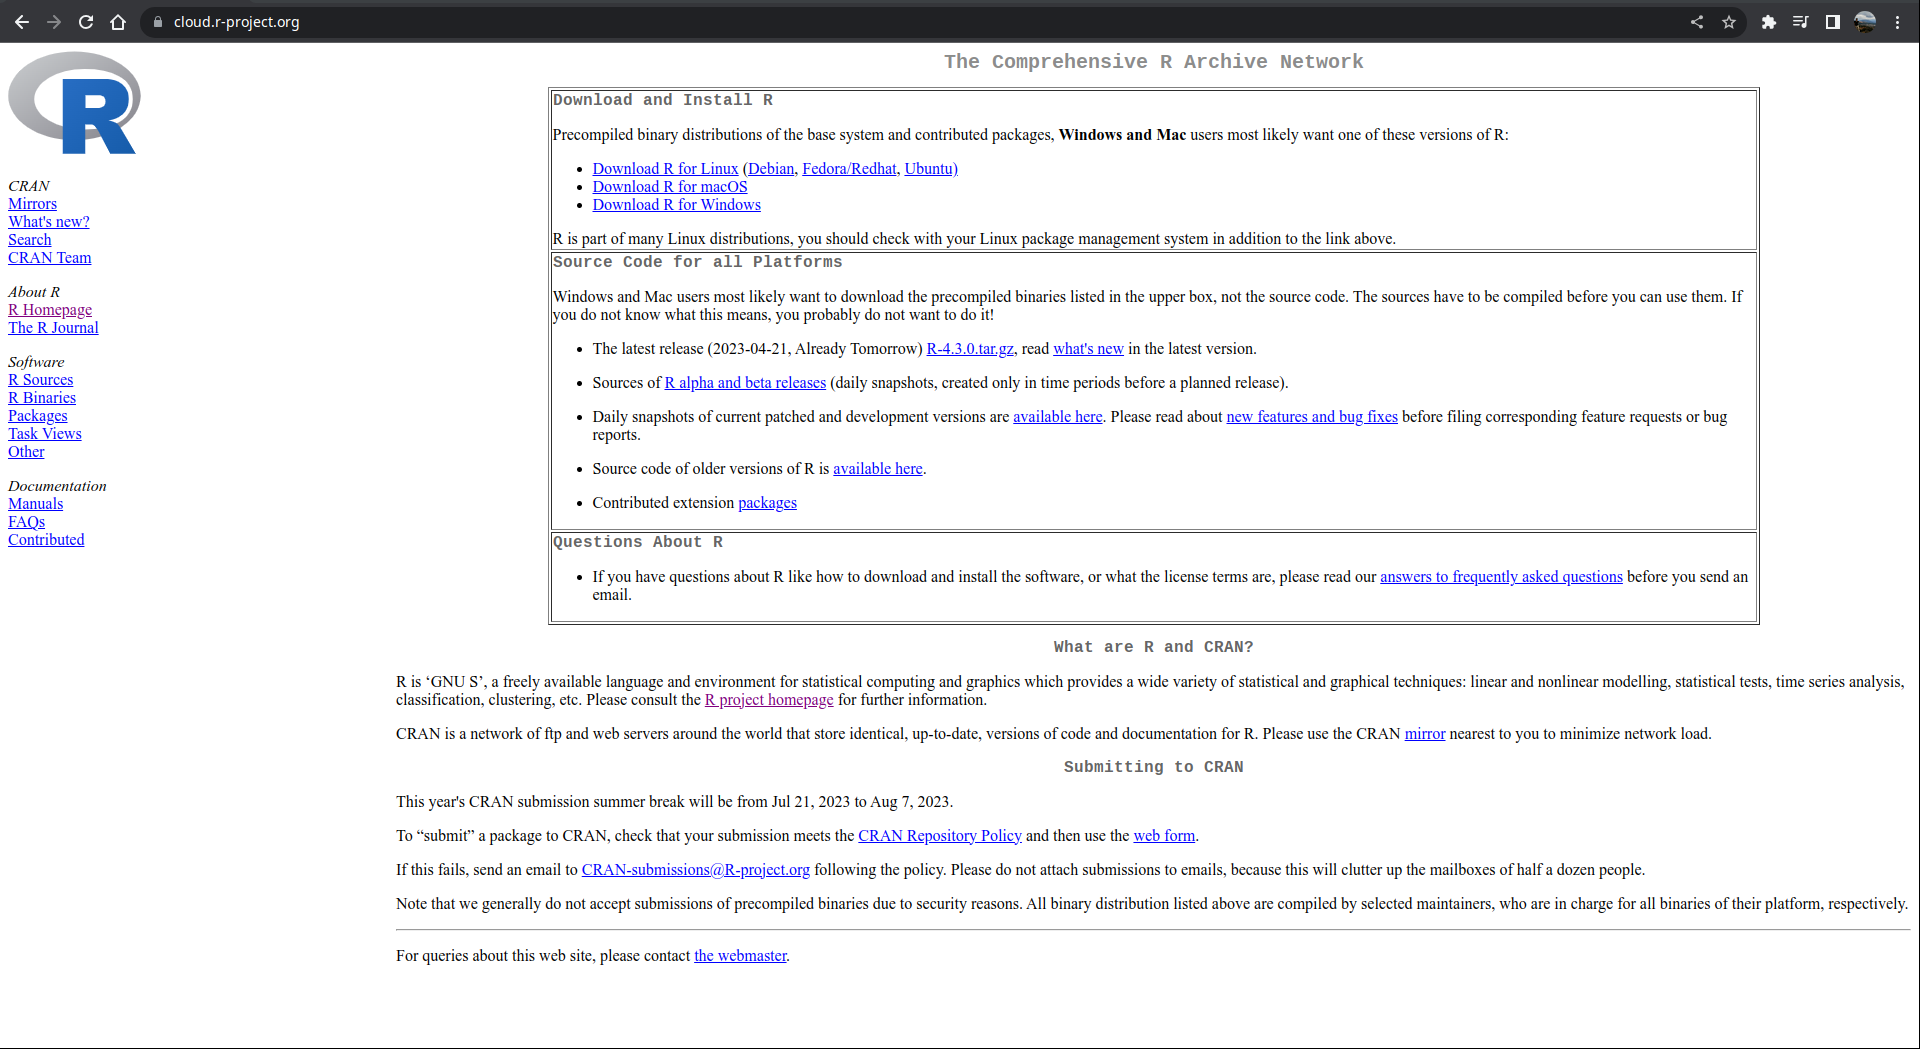
\includegraphics[keepaspectratio]{index_files/figure-html/Screenshot_20230610_222900.png}}

}

\end{figure}%

\subsection{Paso 2. Instalar R en Ubuntu
Linux}\label{paso-2.-instalar-r-en-ubuntu-linux}

Los paquetes para la versión actual de R 4.2 están disponibles para la
mayoría de las versiones estables de Ubuntu Desktop. Sin embargo, solo
la última versión de Soporte a Largo Plazo (LTS) cuenta con soporte
completo. A partir del 2 de mayo de 2022, las versiones compatibles son:

\begin{itemize}
\tightlist
\item
  Jammy Jellyfish (22.04, solo amd64)
\item
  Impish Indri (21.10, solo amd64)
\item
  Focal Fossa (20.04; LTS y solo amd64)
\item
  Bionic Beaver (18.04; LTS)
\item
  Xenial Xerus (16.04; LTS)
\end{itemize}

Ejecuta estas líneas (si eres \texttt{root}, omite \texttt{sudo}) para
informar a Ubuntu sobre los binarios de R en CRAN.

\begin{Shaded}
\begin{Highlighting}[]
\CommentTok{\# Actualizar índices}
\FunctionTok{sudo}\NormalTok{ apt update }\AttributeTok{{-}qq}
\CommentTok{\# Instalar dos paquetes auxiliares necesarios}
\FunctionTok{sudo}\NormalTok{ apt install }\AttributeTok{{-}{-}no{-}install{-}recommends}\NormalTok{ software{-}properties{-}common dirmngr}
\CommentTok{\# Agregar la clave de firma (de Michael Rutter) para estos repositorios}
\CommentTok{\# Para verificar la clave, ejecuta: gpg {-}{-}show{-}keys /etc/apt/trusted.gpg.d/cran\_ubuntu\_key.asc}
\CommentTok{\# Huella digital: E298A3A825C0D65DFD57CBB651716619E084DAB9}
\FunctionTok{wget} \AttributeTok{{-}qO{-}}\NormalTok{ https://cloud.r{-}project.org/bin/linux/ubuntu/marutter\_pubkey.asc }\KeywordTok{|} \FunctionTok{sudo}\NormalTok{ tee }\AttributeTok{{-}a}\NormalTok{ /etc/apt/trusted.gpg.d/cran\_ubuntu\_key.asc}
\CommentTok{\# Agregar el repositorio de R 4.0 de CRAN {-}{-} ajustar \textquotesingle{}focal\textquotesingle{} a \textquotesingle{}groovy\textquotesingle{} o \textquotesingle{}bionic\textquotesingle{} según sea necesario}
\FunctionTok{sudo}\NormalTok{ add{-}apt{-}repository }\StringTok{"deb https://cloud.r{-}project.org/bin/linux/ubuntu }\VariableTok{$(}\ExtensionTok{lsb\_release} \AttributeTok{{-}cs}\VariableTok{)}\StringTok{{-}cran40/"}
\end{Highlighting}
\end{Shaded}

Aquí utilizamos \texttt{lsb\_release\ -cs} para acceder a la versión de
Ubuntu que estás utilizando: ``jammy'', ``impish'', ``focal'',
``bionic'', \ldots{}

Luego, ejecuta

\begin{Shaded}
\begin{Highlighting}[]
\FunctionTok{sudo}\NormalTok{ apt install }\AttributeTok{{-}{-}no{-}install{-}recommends}\NormalTok{ r{-}base}
\end{Highlighting}
\end{Shaded}

\subsection{Obtén más de 5000 paquetes de
CRAN}\label{obtuxe9n-muxe1s-de-5000-paquetes-de-cran}

Ejecuta este comando (como \texttt{root} o agregando \texttt{sudo} como
prefijo) para agregar el repositorio actual de R 4.0 o posterior
`c2d4u':

\begin{Shaded}
\begin{Highlighting}[]
\FunctionTok{sudo}\NormalTok{ add{-}apt{-}repository ppa:c2d4u.team/c2d4u4.0+}
\end{Highlighting}
\end{Shaded}

para agregar el ID de clave de este repositorio, agregar el repositorio
y actualizar el índice. Ahora puedes hacer
\texttt{apt\ install\ -\/-no-install-recommends\ r-cran-rstan} o
\texttt{apt\ install\ -\/-no-install-recommends\ r-cran-tidyverse}
(nuevamente como usuario \texttt{root} o a través de \texttt{sudo}).

\subsection{Paso 3. Descargar RStudio en Ubuntu
Linux}\label{paso-3.-descargar-rstudio-en-ubuntu-linux}

Puedes descargar la última versión de RStudio desde su sitio web
oficial:
\href{https://www.rstudio.com/products/rstudio/download/}{Enlace de
descarga de RStudio}

\begin{quote}
RStudio RStudio es un entorno de desarrollo integrado (IDE) muy popular
para trabajar con R. Proporciona una interfaz gráfica intuitiva y muchas
herramientas útiles para la programación en R.
\end{quote}

\pandocbounded{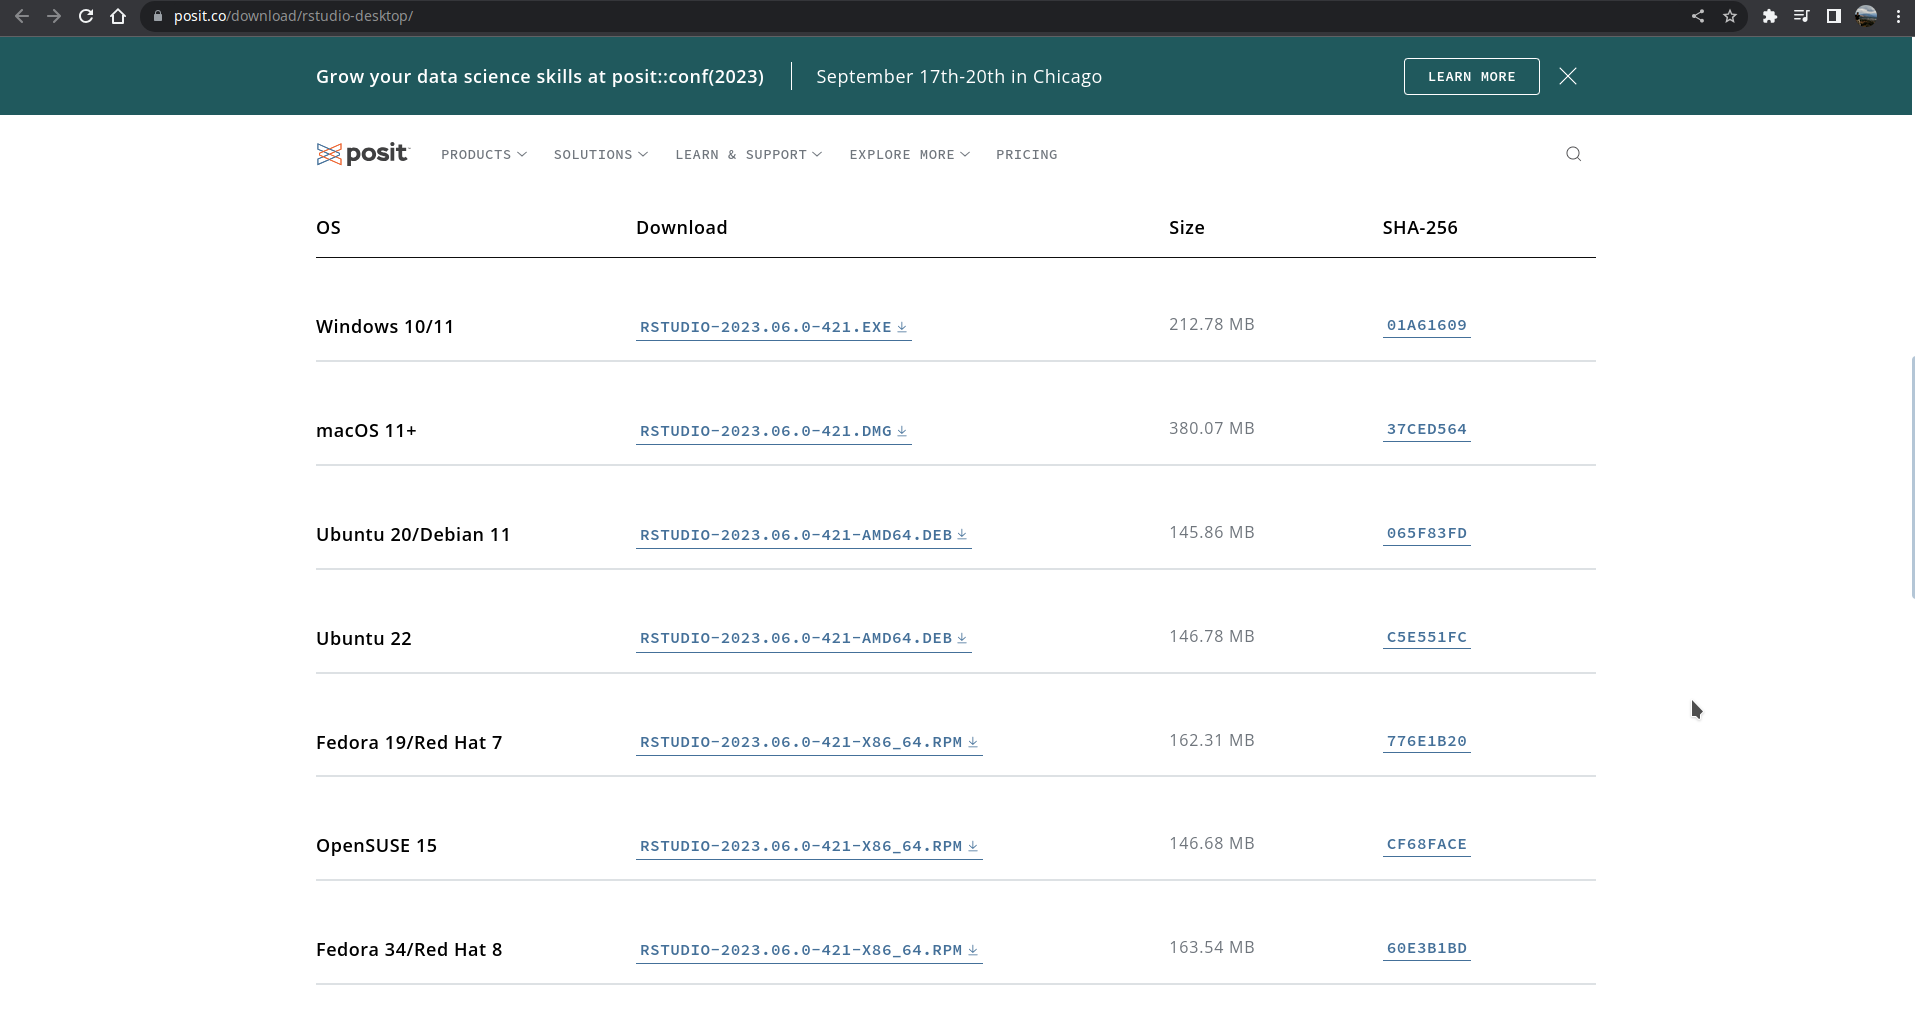
\includegraphics[keepaspectratio]{index_files/figure-html//Screenshot_20230610_224818.png}}

\subsection{Paso 4. Instalar RStudio en Ubuntu
Linux}\label{paso-4.-instalar-rstudio-en-ubuntu-linux}

\subsubsection{Instalar dependencias}\label{instalar-dependencias}

Antes de instalar RStudio, es posible que debas instalar algunas
dependencias en tu sistema. Abre la terminal y ejecuta los siguientes
comandos para instalar las dependencias requeridas:

\begin{Shaded}
\begin{Highlighting}[]
\FunctionTok{sudo}\NormalTok{ apt update}
\FunctionTok{sudo}\NormalTok{ apt install gdebi{-}core}
\end{Highlighting}
\end{Shaded}

Estos comandos actualizarán los repositorios de paquetes y luego
instalarán \texttt{gdebi-core}, una utilidad necesaria para instalar
paquetes \texttt{.deb} de forma sencilla y para resolver dependencias
automáticamente.

\subsubsection{Instalar RStudio}\label{instalar-rstudio}

Una vez que hayas descargado el archivo de instalación de RStudio y
hayas instalado las dependencias necesarias, puedes proceder con la
instalación. Ve al directorio donde descargaste el archivo de
instalación y ejecuta el siguiente comando en la terminal:

\begin{Shaded}
\begin{Highlighting}[]
\FunctionTok{sudo}\NormalTok{ gdebi }\OperatorTok{\textless{}}\NormalTok{nombre\_del\_archivo\_de\_instalación}\OperatorTok{\textgreater{}}\NormalTok{.deb}
\end{Highlighting}
\end{Shaded}

Reemplaza
\texttt{\textless{}nombre\_del\_archivo\_de\_instalación\textgreater{}}
con el nombre real del archivo de instalación descargado.

El comando \texttt{gdebi} instalará RStudio y resolverá automáticamente
las dependencias necesarias.

\subsection{Paso 5. Iniciar RStudio}\label{paso-5.-iniciar-rstudio}

Una vez completada la instalación, puedes iniciar RStudio desde el menú
de aplicaciones de Ubuntu o ejecutando el siguiente comando en la
terminal:

\begin{Shaded}
\begin{Highlighting}[]
\ExtensionTok{rstudio}
\end{Highlighting}
\end{Shaded}

RStudio se abrirá en una ventana separada, lo que te permitirá comenzar
a trabajar con R y aprovechar todas las funciones y características que
ofrece el IDE.

\pandocbounded{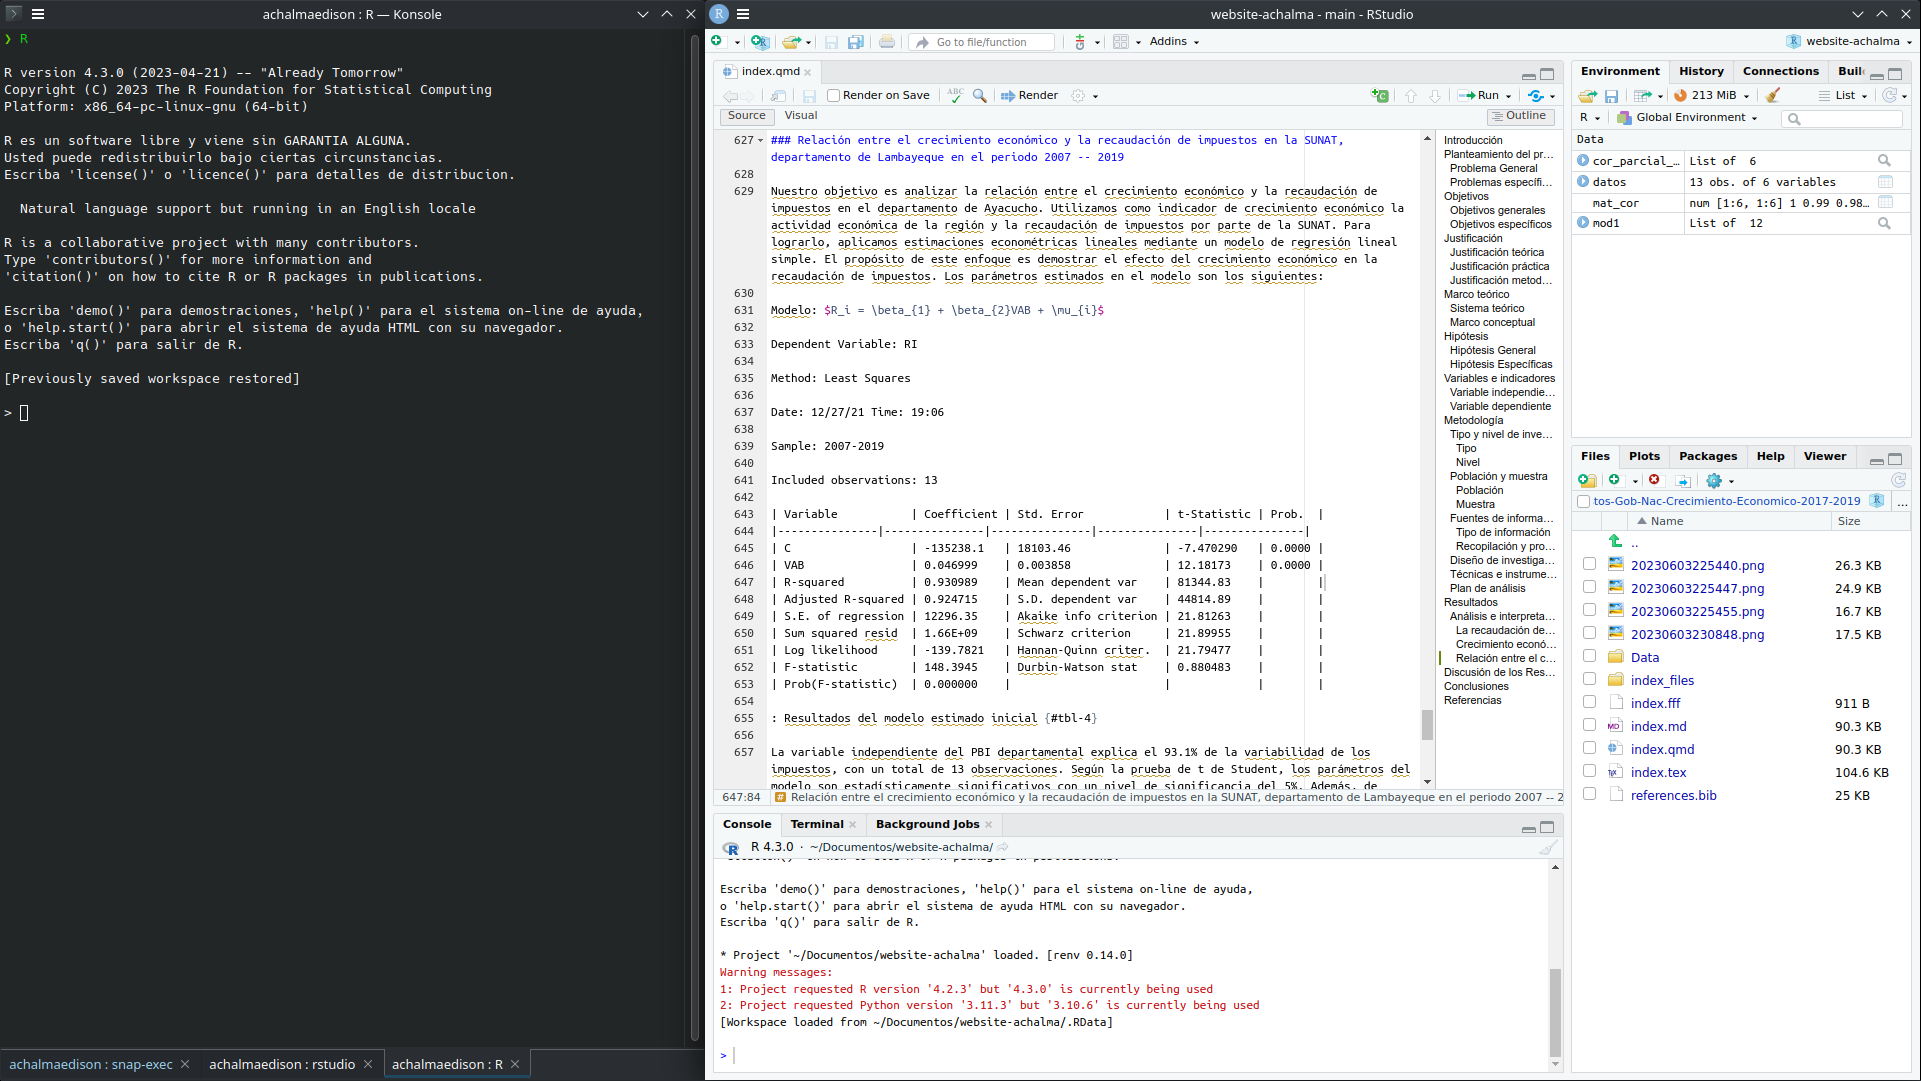
\includegraphics[keepaspectratio]{index_files/figure-html//Screenshot_20230610_231407.png}}

\section{Publicaciones Similares}\label{publicaciones-similares}

Si te interesó este artículo, te recomendamos que explores otros blogs y
recursos relacionados que pueden ampliar tus conocimientos. Aquí te dejo
algunas sugerencias:

\begin{enumerate}
\def\labelenumi{\arabic{enumi}.}
\tightlist
\item
  \href{https://achalmaedison.netlify.app/programacion-software/r/2020-06-10-011-instalacion-de-r/index.pdf}{\faIcon{file-pdf}}
  \href{https://achalmaedison.netlify.app/programacion-software/r/2020-06-10-011-instalacion-de-r}{011
  Instalacion De R}
\item
  \href{https://achalmaedison.netlify.app/programacion-software/r/2020-06-10-012-que-ofrece-r/index.pdf}{\faIcon{file-pdf}}
  \href{https://achalmaedison.netlify.app/programacion-software/r/2020-06-10-012-que-ofrece-r}{012
  Que Ofrece R}
\item
  \href{https://achalmaedison.netlify.app/programacion-software/r/2020-06-10-013-lo-que-debemos-saber-de-r/index.pdf}{\faIcon{file-pdf}}
  \href{https://achalmaedison.netlify.app/programacion-software/r/2020-06-10-013-lo-que-debemos-saber-de-r}{013
  Lo Que Debemos Saber De R}
\item
  \href{https://achalmaedison.netlify.app/programacion-software/r/2021-03-027-01-introduccion-al-programa/index.pdf}{\faIcon{file-pdf}}
  \href{https://achalmaedison.netlify.app/programacion-software/r/2021-03-027-01-introduccion-al-programa}{2021
  03 027 01 Introduccion Al Programa}
\item
  \href{https://achalmaedison.netlify.app/programacion-software/r/2021-04-05-02-manipulacion-de-datos/index.pdf}{\faIcon{file-pdf}}
  \href{https://achalmaedison.netlify.app/programacion-software/r/2021-04-05-02-manipulacion-de-datos}{02
  Manipulacion De Datos}
\item
  \href{https://achalmaedison.netlify.app/programacion-software/r/2021-04-12-03-visualizacion-de-datos/index.pdf}{\faIcon{file-pdf}}
  \href{https://achalmaedison.netlify.app/programacion-software/r/2021-04-12-03-visualizacion-de-datos}{03
  Visualizacion De Datos}
\item
  \href{https://achalmaedison.netlify.app/programacion-software/r/2022-11-07-04-modelo-de-machine-learning-i-analisis-exploratorio/index.pdf}{\faIcon{file-pdf}}
  \href{https://achalmaedison.netlify.app/programacion-software/r/2022-11-07-04-modelo-de-machine-learning-i-analisis-exploratorio}{04
  Modelo De Machine Learning I Analisis Exploratorio}
\item
  \href{https://achalmaedison.netlify.app/programacion-software/r/2022-11-14-05-modelo-de-machine-learning-ii-modelo-de-clasificacion/index.pdf}{\faIcon{file-pdf}}
  \href{https://achalmaedison.netlify.app/programacion-software/r/2022-11-14-05-modelo-de-machine-learning-ii-modelo-de-clasificacion}{05
  Modelo De Machine Learning Ii Modelo De Clasificacion}
\item
  \href{https://achalmaedison.netlify.app/programacion-software/r/2022-11-21-06-modelo-de-machine-learning-iii-modelo-de-regresion/index.pdf}{\faIcon{file-pdf}}
  \href{https://achalmaedison.netlify.app/programacion-software/r/2022-11-21-06-modelo-de-machine-learning-iii-modelo-de-regresion}{06
  Modelo De Machine Learning Iii Modelo De Regresion}
\item
  \href{https://achalmaedison.netlify.app/programacion-software/r/2022-11-28-07-modelo-de-machine-learning-iv-tex-mining/index.pdf}{\faIcon{file-pdf}}
  \href{https://achalmaedison.netlify.app/programacion-software/r/2022-11-28-07-modelo-de-machine-learning-iv-tex-mining}{07
  Modelo De Machine Learning Iv Tex Mining}
\end{enumerate}

Esperamos que encuentres estas publicaciones igualmente interesantes y
útiles. ¡Disfruta de la lectura!






\end{document}
